\documentclass[10pt,conference]{IEEEtran}

\usepackage[utf8]{inputenc}
\usepackage{cite}
\usepackage{hyperref}
\usepackage{graphicx}	% For figure environment


\begin{document}
\title{Characterization of turbulent flows in tokamaks}

\author{
  Julien Hu, Matthieu Masouyé and Sébastien Ollquist\\
  \textit{Department of Computer Science, EPFL, Switzerland}
}

\maketitle
\thispagestyle{plain}
\pagestyle{plain}

\begin{abstract}
    The goal of this project was to use machine learning to analyze GPI measures and estimate the Z-axis velocity of the structures.\par 
    To do that, we have used a convolutional neural network (CNN) on a resnet 3d architecture, with the help of a synthetic dataset we generated ourselves.\par
    We were able to successfully train and optimize a CNN for each dataset, and overall we were able to have good estimation of the speeds; however, time constraints prevented us from going as far as we would have liked.
\end{abstract}

\section{Introduction}
A tokamak is a type of plasma generator, inside which plasma turns at very high speeds. The plasma is confined in the shape of a torus via magnetic fields. At the edges of this field, it separates from the flow in a turbulent fashion; this is called the shear layer. These turbulences might create "blobs" of plasma, that can be ejected at high speed.\par 
Gas Puff Imaging (GPI) is a technique used to study these turbulences: it consists in launching a puff of neutral gas near the shear layer, to generate light emissions when mixing up with the plasma and thus allowing imaging of the turbulent structures. These images are cross-sections of the plasma, with two axis: an $r$-axis perpendicular to the wall of the torus, and a $z$-axis going vertically and parallel from the $r$-axis, along side the shear layer.\par
GPI analysis is an ongoing task, and can yield important results. The Swiss Plasma Center lab at EPFL was interested in the new possibilities machine learning could bring, and together we worked to test how well a neural network could analyze these images.\par
 
The primary objective was to measure the $z$-axis velocities of the moving, turbulent structures captured by GPI. We quickly decided to go for a convolutional neural network working on sequences of frames, as it seems a good approach for complex tasks and apt for image sequence analysis and velocity estimation \cite{velocitycnn}.

 

\section{Data and preprocessing}

\subsection{Real Data Description}
The labeled data was given to us from the lab in pickle files, inside which there are the following sets:
\begin{enumerate}
  \item \texttt{shot} the shot number.
  \item \texttt{t\_window} an array of timestamps at which the frames were measured, in seconds
  \item \texttt{brt\_arr} a 3D-array (of 12x10x$l$ where $l$ is the length of \texttt{t\_window}) of G.P.I. measures, corresponding to the brightness of each 12 by 10 frames, measured in $mW/cm^2/ster$
  \item \texttt{r\_arr} the array of $r$-coordinate of each view, in meters.
  \item \texttt{z\_arr} the similar array of $z$-coordinate of each view, also in meters.
  \item \texttt{vz\_from\_wk} the vertical speed for each column of data, in $km/s$.
  \item \texttt{vz\_err\_from\_wk} the error margin in the estimation of vz
  \item \texttt{col\_r} the average $r$-coordinate of each column.
\end{enumerate}
Due to the measurement method, four specific "pixels" of \texttt{brt\_arr} are set to NaN permanently. The \texttt{r\_arr} and \texttt{z\_arr} describe the exact position of each pixel of \texttt{brt\_arr} in a 2d space, as they are not perfectly spaced. \texttt{vz\_from\_wk} will constitute the labels for the algorithm.\par
Importantly, there are 13 values in \texttt{vz\_from\_wk}, \texttt{vz\_err\_from\_wk} and \texttt{col\_r} while there are only 12 columns per frames: this is because the shear layer we want to calculate is inside one of the columns, which means this column will have flows going both ways. Thus, this column will have two speeds associated to it. This also means that \texttt{col\_r} has two identical values, as they concern the same column.\par
Note that it wasn't possible for the lab to provide good estimates of these two speeds in all datasets, and the 13th column will be set to NaN if they couldn't get an accurate estimation. 
Additionnally, the direction of the plasma relative to the shear layer is consistent: the left side always has plasma going down (i.e. negative values), while the right side always going up (i.e. positive values). 

\subsection{Synthetic Data Description}
We have decided to generate artificial data mainly for two reasons: first is that the real dataset would take some time for the lab to prepare; and more importantly it would give us a controlled environment with no noise or imprecision in the labels, so that we could use this dataset to evaluate different architectures.\par
With the help of the lab directors, we could generate this in the following way: we draw a large canvas (by default 480x480), and spawn in random gaussian arrays of varying small sizes (around 264 arrays of 100 to 260 pixels wide). A ratio of these arrays are also set to negative values. To draw a frame, all the arrays are summed in the canvas, and values are limited to between 0 and 255 to stay in an 8 bit grayscale. Then, a smaller window at the center is taken and downsized until it reaches the final size of 10x12, same as the real data.\par
To update the position of these arrays, they are attributed a vertical speed given their horizontal coordinate, and at each frame their new positions are calculated by adding this speed. The function used to assign these speeds is the hyperbolic tangent $\tanh$, with several settings to tweak its behaviour. To get the labels, we can simply average this speed function over each column of the final window.\par
Everytime the script is run, it will generate a new folder inside \texttt{data/}, where it will put the final frames, the labels, and various other information for debuging and for reproducibility purposes (like a speedplot, a list of settings, and a video of all the frames).
At the beginning of the script there is a list of variables used as settings to tweak the behaviour of the generated dataset.
 
\begin{figure}
  \centering
  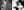
\includegraphics[scale=4]{images/comparison.png}
  \caption{Real image on the left, synthetic image on the right}
\end{figure}
 
This method gets reasonably close to how the real data looks like. In the precedent description, we have overseen a few simplifications in the behaviour of the synthetic dataset. For instance, the shear layer is always vertical but the real data's shear layer is slightly curved. Another important distinction is that the speed of the structures aren't only along side the $z$-axis in the plasma. Simulating these aspects has been judged too complex, and instead some shortcuts like the negative gaussians are there to try and mitigate this. Overall, the lab seemed satisfied with these synthetic datas.
 


\subsection{Data Manipulation and Preprocessing}
We have implemented two different data loaders, that are used to organize and load real or synthetic data into the CNN.\par
Both data loaders organize the frames into 2000-frames datapoints (10x12x2000 values), and shuffle these datapoints using a fixed seed to homogenize the different scenarios. These datapoints are separated into 3 datasets: one for training, one for validation, and one for testing, with default ratios of 64\%, 16\% and 20\% respectively.\par
The last transformation these datapoints need is to be converted from a 1-channel greyscale to 3-channel, to be compatible with the architectures we used. This was done simply by duplicating the single channel across the two others.\par
The differences between the two data loaders are where and how they fetch the frames, as they are stored in a different way on disk. Moreover, the dataloader working on real data has to rescale the values of the measures to be 8-bit greyscale images instead of raw brightness measures. This isn't a problem for the synthetic dataloader as the synthetic data was already generated in a convenient way.

Due to time constraints, we only could use part of all the sets for the real data: \texttt{t\_window}, \texttt{r\_arr}, \texttt{z\_arr} and \texttt{vz\_err\_from\_wk} were not taken into consideration for our algorithm. Moreover, we had to ignore datasets where the 13th column was missing as described in the real data description, as that would have required us to redo our approach completely.\par
Finally, we chose to work with inputs of 2000 images, as more images was pushing the limits of our computers in terms of time and memory. The lab estimated that an entire structure would take approximately 18'000 frames to cross the image completely. 2'000 frames should ensure it moves at least one pixel, as the images has a height of 10 pixels.\par


\section{Model training}
 
\subsection{The CNN architectures}
To perform our regression task, we have decided to work on the architectures defined for video classification in PyTorch, for simplicity and efficiency: we trust the models have been optimized and tested, and it would be easier and safer to implement them rather than develop our own network. The models used are: \textit{ResNet 3D}, \textit{ResNet Mixed Convolution} and \textit{ResNet (2+1)D} \cite{resnets}. ResNet is a classic neural network that helps solving computer vision tasks \cite{hara3dcnns}. As we have to analyze a sequence of images, this model is appropriate for our problem.\par
These networks consist of multiple processing layers that perform different operations to process the input, extract and recognise its key features (measurable property or characteristic), and predict the desired outputs. These layers are:
\begin{itemize}
  \item The convolutional layer, in which features from input images or feature maps are extracted by applying filters, each composed of small kernels.
  \item The pooling layer, that is similar to the convolutional layer, but performs a specific function, such as taking the maximum or average value in a region, to reduce the complexity and amount of computation of the network 
  \item The fully connected layer, where after all the necessary computation is done, the network regroups all informations from the final feature maps, and generates the output.
\end{itemize}

The main difference between the three architectures lies in the convolutional layers, where filters are applied distinctively:
\begin{itemize}
  \item ResNet 3D performs a 3D convolution, the 3D filters are convolved over both time and space dimensions.
  \item ResNet Mixed Convolution starts with 3D convolution, then at later layers, uses 2D convolution, as at higher level of abstraction, motion or temporal modeling may not be necessary.
  \item ResNet (2+1)D seperates the 3D convolution into two steps, a 2D convolution in the space dimension followed by a 1D convolution in time, to reduce the computation cost \cite{spacetimeconv}.
\end{itemize}

\subsection{The training procedure}
The main goal we want to achieve when training a model is preparing it sufficiently with randomly generated data in order for it to be ready for the real data. In our case, we start training it on the synthetic data we generated so that we can get a good impression of how well it performs. Only then, we can start training it on the real data, and optimize with both datasets.\par
The training loop consists of two main phases:
\begin{enumerate}
    \item {\bf The training phase} In this phase, the model learns how to recognize the key features and where they are, and will update its weights (learnable parameters) with its performance on the dataset. The inputs traverse the whole network, and the model will predict the values for the output, and compare with the labels. Then, the gradients are propagated and the model updates its weights. Note that it only learns with the training set. After the entire set is passed through the network, it then proceeds to the next phase
    \item {\bf The validation phase} In this phase, the model simply predicts the output for the validation set, and we compute the loss. This part is to give an estimation how good the model performs at each iteration, to detect any signs of overfitting, and tune hyperparameters later.
\end{enumerate}
Each step is repeated for 30 epochs. The best validation results are used to compare different instances of the model and finetune the hyperparameters. After optimizing and selecting the best performing model, it is then tested on the testing set, which contains data that the model has never been executed with. The testing phase is only to provide us with an evaluation of the final model.\par
The loss function used to evaluate the model is the MSE (Mean Square Error) loss function, as it is the most commonly used function for regression tasks. 
As for the optimizer, we decide to choose the optimizer SGD. We tested with Adam, but the model struggled to converge, and resulted in worse losses.
 
\subsection{Finding the correct architecture}
To find the most suitable model for our task, we decided to train and evaluate with our synthetic dataset, as we only had that available at the time. We see from the last validation results from table \ref{table:comparisonLoss}, that ResNet 3D offers the best results. Moreover, while training the models afterwards, our computers were unable to handle the ResNet MixedConv and ResNet 2+1D, as the memory load is too heavy with some set of hyperparameters, and would restrain us for optimization. We therefore decide to use and optimize ResNet 3D.  

\begin{table}[h!]
\centering
 \begin{tabular}{|c | c |} 
 \hline
    Architecture & Validation loss \\  
 \hline\hline
    ResNet 3D & 1.021\\ 
 \hline
    ResNet MixedConv & 3.792\\
 \hline
    ResNet 2+1D & 3.284\\
 \hline
\end{tabular}
\caption{Last validation results for the architectures after 30 epochs.}
\label{table:comparisonLoss}
\end{table}

To finetune our model, we decided to start by training our model on the synthetic dataset, to have a first impression on how the model will behave and which hyperparameters to optimize. The hyperparameters we chose to finetune are :
\begin{itemize}
  \item The learning rate \textit{lr}, which describes how fast the model adapts to the problem, how much should it update its weights based on the estimated error. Choosing a learning rate that is too high can cause the model to converge too quickly to a sub-optimal solution or overfit the training data, while a too low learning rate results in a long training process, or can even cause the model to be stuck.
  \item \textit{batch\_size}, which defines the number of samples that will be trained at the same time, and affects how the gradient is calculated when correcting the weights. In short, bigger batches means the gradient should fluctuate less and be more accurate, at the expense of memory required. But it doesn't necessarily means a better model, as a noisier gradient might lead to a more robust model.
\end{itemize}
 
%The smaller the batch the less accurate the estimate of the gradient will be. In the figure below, you can see that the direction of the mini-batch gradient (green color) fluctuates much more in comparison to the direction of the full batch gradient (blue color). 

\section{Results}
\begin{table}
    \centering
    \begin{tabular}{|c || c | c | c | c | c | c| c | c |} 
        \hline
         & 0.005 & 0.01 & 0.02 & 0.03 & 0.04 & 0.05 & 0.06 \\  
        \hline\hline
        2 & 3.77 & 2.81 & 1.50 & 2.54 &  &  &\\ 
        \hline
        4 & S & M &  & J &  &  &\\
        \hline
        8 & (S) &  &  &  &  &  &\\
        \hline
        16 &  &  & 5.76 & 4.02 & 3.97 & 3.12 & 4.00\\
        \hline
    \end{tabular}
    \caption{Batch size (column) vs learning rate (rows) on synthetic data}
\end{table}

\begin{table}
    \centering
     \begin{tabular}{|c || c | c | c | c | c | c| } 
     \hline
       & 0.005 & 0.01 & 0.02 & 0.03 & 0.04 \\  
     \hline\hline
     2 & 21.20 & 18.52 &  19.21 &  20.69 & 27.09\\ 
     \hline
     4 & 20.45 & 19.64 & 21.29 &  21.50 & 21.54 \\
     \hline
     8 &  & 18.91 & 18.90 &  18.21 & 19.80 \\
     \hline
     16 &  & 19.89 & 18.50 &  19.35 & \\
     \hline
    \end{tabular}
    \caption{Batch size (column) vs learning rate (rows) on the real data}
\end{table}


\section{Conclusion}

\bibliographystyle{IEEEtran}
\bibliography{project2}

\end{document}